% !TeX program = pdfLaTeX
\documentclass[12pt]{article}
\usepackage{amsmath}
\usepackage{graphicx,psfrag,epsf}
\usepackage{enumerate}
\usepackage{natbib}
\usepackage{textcomp}
\usepackage[hyphens]{url} % not crucial - just used below for the URL
\usepackage{hyperref}
\providecommand{\tightlist}{%
  \setlength{\itemsep}{0pt}\setlength{\parskip}{0pt}}

%\pdfminorversion=4
% NOTE: To produce blinded version, replace "0" with "1" below.
\newcommand{\blind}{0}

% DON'T change margins - should be 1 inch all around.
\addtolength{\oddsidemargin}{-.5in}%
\addtolength{\evensidemargin}{-.5in}%
\addtolength{\textwidth}{1in}%
\addtolength{\textheight}{1.3in}%
\addtolength{\topmargin}{-.8in}%

%% load any required packages here


\usepackage{color}
\usepackage{fancyvrb}
\newcommand{\VerbBar}{|}
\newcommand{\VERB}{\Verb[commandchars=\\\{\}]}
\DefineVerbatimEnvironment{Highlighting}{Verbatim}{commandchars=\\\{\}}
% Add ',fontsize=\small' for more characters per line
\usepackage{framed}
\definecolor{shadecolor}{RGB}{248,248,248}
\newenvironment{Shaded}{\begin{snugshade}}{\end{snugshade}}
\newcommand{\AlertTok}[1]{\textcolor[rgb]{0.94,0.16,0.16}{#1}}
\newcommand{\AnnotationTok}[1]{\textcolor[rgb]{0.56,0.35,0.01}{\textbf{\textit{#1}}}}
\newcommand{\AttributeTok}[1]{\textcolor[rgb]{0.77,0.63,0.00}{#1}}
\newcommand{\BaseNTok}[1]{\textcolor[rgb]{0.00,0.00,0.81}{#1}}
\newcommand{\BuiltInTok}[1]{#1}
\newcommand{\CharTok}[1]{\textcolor[rgb]{0.31,0.60,0.02}{#1}}
\newcommand{\CommentTok}[1]{\textcolor[rgb]{0.56,0.35,0.01}{\textit{#1}}}
\newcommand{\CommentVarTok}[1]{\textcolor[rgb]{0.56,0.35,0.01}{\textbf{\textit{#1}}}}
\newcommand{\ConstantTok}[1]{\textcolor[rgb]{0.00,0.00,0.00}{#1}}
\newcommand{\ControlFlowTok}[1]{\textcolor[rgb]{0.13,0.29,0.53}{\textbf{#1}}}
\newcommand{\DataTypeTok}[1]{\textcolor[rgb]{0.13,0.29,0.53}{#1}}
\newcommand{\DecValTok}[1]{\textcolor[rgb]{0.00,0.00,0.81}{#1}}
\newcommand{\DocumentationTok}[1]{\textcolor[rgb]{0.56,0.35,0.01}{\textbf{\textit{#1}}}}
\newcommand{\ErrorTok}[1]{\textcolor[rgb]{0.64,0.00,0.00}{\textbf{#1}}}
\newcommand{\ExtensionTok}[1]{#1}
\newcommand{\FloatTok}[1]{\textcolor[rgb]{0.00,0.00,0.81}{#1}}
\newcommand{\FunctionTok}[1]{\textcolor[rgb]{0.00,0.00,0.00}{#1}}
\newcommand{\ImportTok}[1]{#1}
\newcommand{\InformationTok}[1]{\textcolor[rgb]{0.56,0.35,0.01}{\textbf{\textit{#1}}}}
\newcommand{\KeywordTok}[1]{\textcolor[rgb]{0.13,0.29,0.53}{\textbf{#1}}}
\newcommand{\NormalTok}[1]{#1}
\newcommand{\OperatorTok}[1]{\textcolor[rgb]{0.81,0.36,0.00}{\textbf{#1}}}
\newcommand{\OtherTok}[1]{\textcolor[rgb]{0.56,0.35,0.01}{#1}}
\newcommand{\PreprocessorTok}[1]{\textcolor[rgb]{0.56,0.35,0.01}{\textit{#1}}}
\newcommand{\RegionMarkerTok}[1]{#1}
\newcommand{\SpecialCharTok}[1]{\textcolor[rgb]{0.00,0.00,0.00}{#1}}
\newcommand{\SpecialStringTok}[1]{\textcolor[rgb]{0.31,0.60,0.02}{#1}}
\newcommand{\StringTok}[1]{\textcolor[rgb]{0.31,0.60,0.02}{#1}}
\newcommand{\VariableTok}[1]{\textcolor[rgb]{0.00,0.00,0.00}{#1}}
\newcommand{\VerbatimStringTok}[1]{\textcolor[rgb]{0.31,0.60,0.02}{#1}}
\newcommand{\WarningTok}[1]{\textcolor[rgb]{0.56,0.35,0.01}{\textbf{\textit{#1}}}}


\begin{document}


\def\spacingset#1{\renewcommand{\baselinestretch}%
{#1}\small\normalsize} \spacingset{1}


%%%%%%%%%%%%%%%%%%%%%%%%%%%%%%%%%%%%%%%%%%%%%%%%%%%%%%%%%%%%%%%%%%%%%%%%%%%%%%

\if0\blind
{
  \title{\bf Calendar-based graphics for visualizing people's daily schedules}

  \author{
        Earo Wang \\
    Department of Econometrics and Business Statistics, Monash University\\
     and \\     Dianne Cook \\
    Department of Econometrics and Business Statistics, Monash University\\
     and \\     Rob J Hyndman \\
    Department of Econometrics and Business Statistics, Monash University\\
      }
  \maketitle
} \fi

\if1\blind
{
  \bigskip
  \bigskip
  \bigskip
  \begin{center}
    {\LARGE\bf Calendar-based graphics for visualizing people's daily schedules}
  \end{center}
  \medskip
} \fi

\bigskip
\begin{abstract}
Calendars are broadly used in society to display temporal information and events. This paper describes a new calendar display for plotting data, that includes a layout algorithm with many options, and faceting functionality. The functions use modular arithmetic on the date variable to restructure the data into a calendar format. The user can apply the grammar of graphics to create plots inside each calendar cell, and thus the displays synchronize neatly with \textbf{ggplot2} graphics. The motivating application is studying pedestrian behavior in Melbourne, Australia, based on counts which are captured at hourly intervals by sensors scattered around the city. Faceting by the usual features such as day and month, is insufficient to examine the behavior. Making displays on a monthly calendar format helps to understand pedestrian patterns relative to events such as work days, weekends, holidays, and special events. The functions for the calendar algorithm are available in the R package \textbf{sugrrants}.
\end{abstract}

\noindent%
{\it Keywords:} data visualization, statistical graphics, time series, grammar of graphics, R
\vfill

\newpage
\spacingset{1.45} % DON'T change the spacing!

\hypertarget{introduction}{%
\section{Introduction}\label{introduction}}

A new method for organizing and visualizing temporal data, collected at sub-daily intervals, into a calendar layout is developed. The format is created using modular arithmetic, giving a restructuring of the data that can then be integrated into a data pipeline. The core component of the pipeline is to visualize the resulting data using the grammar of graphics \citep{wilkinson2006grammar, wickham2009ggplot2}, as used in \textbf{ggplot2} \citep{R-ggplot2}, where plots are defined as a functional mapping from variables in the data to graphical elements. The data restructuring approach is consistent with the tidy data principles available in the \textbf{tidyverse} suite of tools \citep{R-tidyverse}. The methods are implemented in a new R package called \textbf{sugrrants} \citep{R-sugrrants}.

The purpose of the calendar-based visualization is to provide insights into human activities, especially relative to events such as work days, weekends, holidays, and special events. This work was originally motivated by studying foot traffic in the city of Melbourne, Australia \citep{ped}. There are many sensors installed across the inner-city area, that count pedestrians every hour (Figure \ref{fig:ped-map}). Data from 43 sensors in 2016 is analyzed here. This data can shed light on people's daily rhythms, and assist the city administration and local businesses with event planning and operational management. Patterns relative to special events (such as public holidays and recurring cultural/sporting events) would be worth studying in comparison to regular days, but conventional displays of time series data may bury this detail.

A routine examination of the data would involve constructing a time series plot to examine the temporal patterns. The faceted plots in Figure \ref{fig:time-series-plot} give an overall picture of the foot traffic at three different sensors in 2016. Further faceting by day of the week (Figure \ref{fig:facet-time}) provides a better view of the daily and sub-daily (hourly) pedestrian patterns. Flagstaff Station has a strong commuter pattern, with peaks in the morning and evening, and no pedestrians on the weekend. Around the State Library there are pedestrians walking around during the day, and an unusually large number on one Saturday night and Sunday morning. Birrarung Marr has a varied pedestrian pattern, with very different numbers of people on different days and times.

Faceting, initially called trellis displays \citep{becker_visual_1996}, is an example of a small multiple \citep{tufte1983visual}, where different subsets of the same data are displayed across one or more conditioning variables. It allows the comparison of subsets. Faceting can also be thought of as a simple ensemble graphic \citep{unwin_ensemble_2018}. It is a homogeneous collection of plots, whereas the ensemble graphics broadly organize related plots for a data set together into one display.

\begin{figure}

{\centering 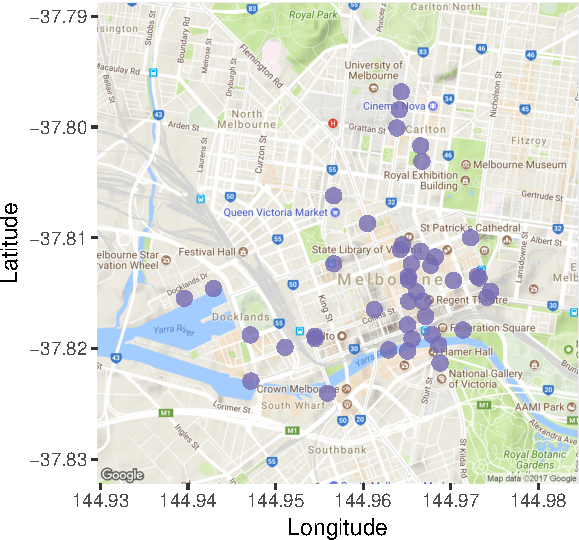
\includegraphics[width=0.7\linewidth]{figure/ped-map-1} 

}

\caption{Google map of the Melbourne city area, grey dots indicate sensor locations. The three locations highlighted will be analyzed in the paper: the State Library is a public library; Flagstaff Station is a train station, closed on non-work days; Birrarung Marr is an outdoor park hosting many cultural and sports events.}\label{fig:ped-map}
\end{figure}



\begin{figure}

{\centering 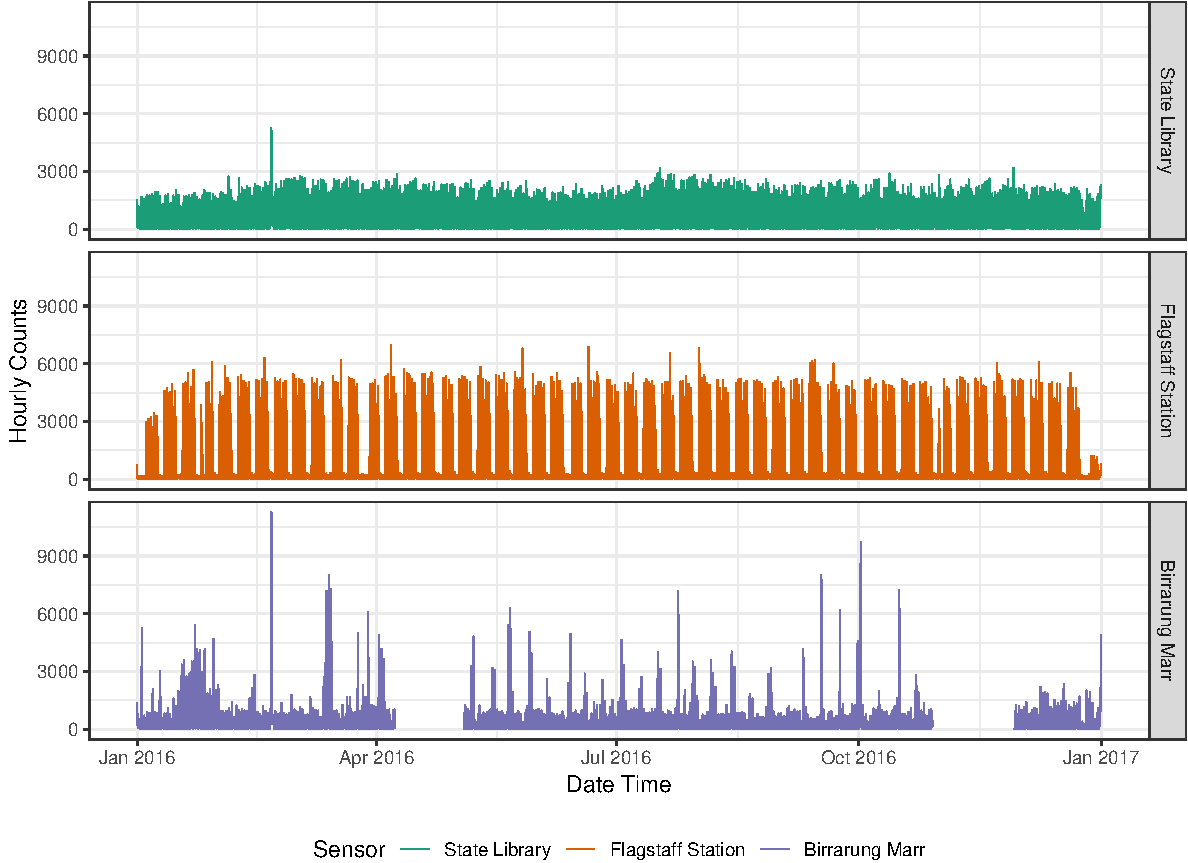
\includegraphics[width=\textwidth]{figure/time-series-plot-1} 

}

\caption{Time series plots showing 2016 pedestrian counts, measured by three different sensors in the city of Melbourne. Small multiples of lines show that the foot traffic varies at one location to another. The spike in counts at the State Library corresponds to the timing of the event ``White Night'', where there were many people taking part in activities in the city throughout the night. A relatively persistent pattern repeats from one week to another at Flagstaff Station. Birrarung Marr looks rather noisy and spiky, with several runs of missing records.}\label{fig:time-series-plot}
\end{figure}



\begin{figure}

{\centering 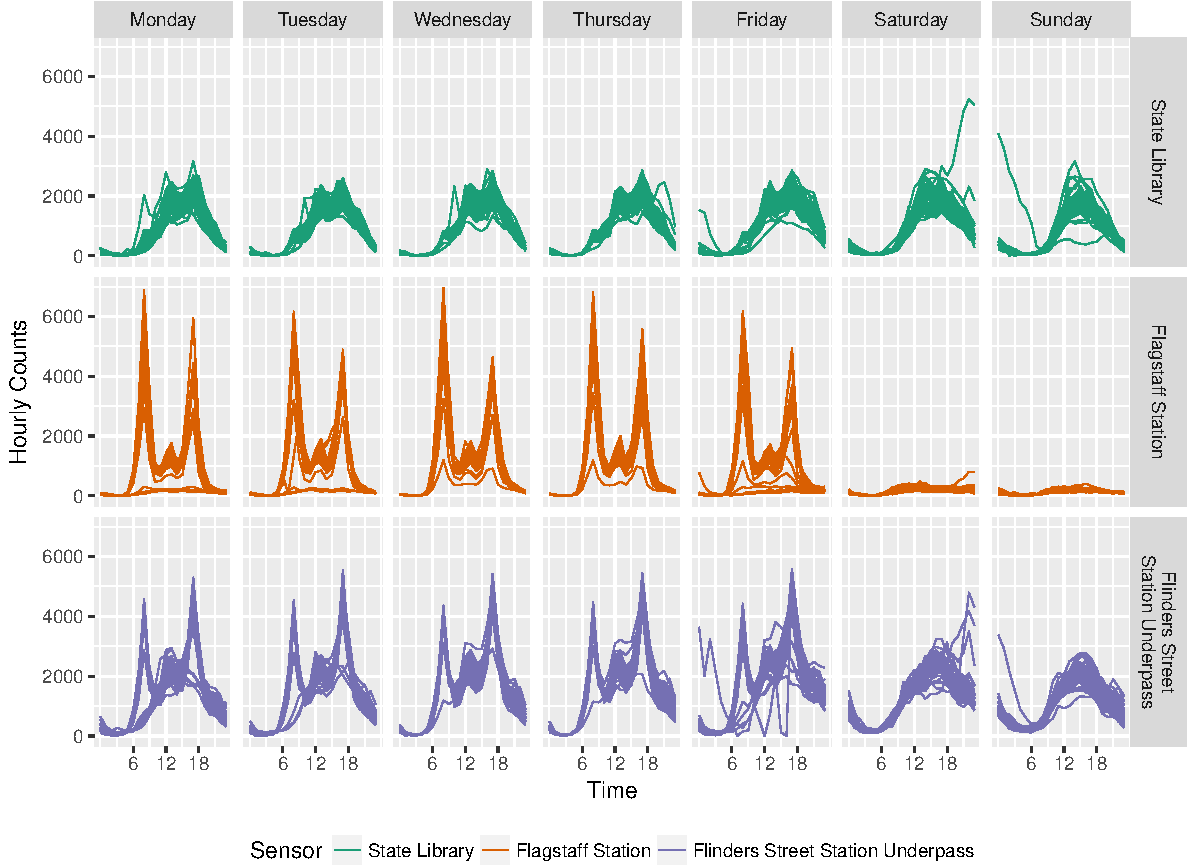
\includegraphics[width=\textwidth]{figure/facet-time-1} 

}

\caption{Hourly pedestrian counts for 2016, faceted by sensors, and days of the week. The focus is on time of day and day of week across the sensors. Daily commuter patterns at Flagstaff Station, the variability of the foot traffic at Birrarung Marr, and the consistent pedestrian behavior at the State Library, can be seen.}\label{fig:facet-time}
\end{figure}



The work is inspired by \citet{Wickham2012glyph}, which uses modular arithmetic to display spatio-temporal data as glyphs on maps. It is also related to recent work by \citet{R-geofacet} which provides methods in the \textbf{geofacet} R package to arrange data plots into a grid, while preserving the geographical position. Both of these show data in a spatial context.

In contrast, calendar-based graphics unpack the temporal variable, at different resolutions, to digest multiple seasonalities and special events. There are some existing works in this area. For example, \citet{VanWijkCluster1999} developed a calendar view of the heatmap to represent the number of employees in the work place over a year, where colors indicate different clusters derived from the days. It contrasts weekdays and weekends, highlights public holidays, and presents other known seasonal variation such as school vacations, all of which have influence over the turn-outs in the office. Some variants of calendar-based heatmaps have been implemented in R packages: \textbf{TimeProjection} \citep{R-TimeProjection}, \textbf{ggTimeSeries} \citep{R-ggTimeSeries}, and \textbf{ggcal} \citep{R-ggcal}. However, these techniques are limited to color-encoding graphics and are unable to use time scales smaller than a day. Time of day, which serves as one of the most important aspects in explaining substantial variations arising from the pedestrian sensor data, will be neglected through daily aggregation. Color-encoding is also low on the hierarchy of optimal variable mapping \citep{cleveland1984graphical, lam2007overview}.

The proposed algorithm goes beyond the calendar-based heatmap. The approach is developed with three conditions in mind: (1) to display time-of-day variation in addition to longer temporal components such as day-of-week and day-of-year; (2) to incorporate lines and other types of glyphs into the graphical toolkit for the calendar layout; (3) to accentuate unusual patterns, such as those related to special events, for viewers. The proposed algorithm has been implemented in the \texttt{frame\_calendar()} and \texttt{facet\_calendar()} functions in the \textbf{sugrrants} package using R.

The remainder of the paper is organized as follows. Section \ref{sec:algorithm} details the construction of the calendar layout in depth. It describes the algorithms of data transformation (Section \ref{sec:transformation}), the available options (Section \ref{sec:opt}), variations of its usage (Section \ref{sec:variations}), and the full faceting extension equipped with formal labels and axes (Section \ref{sec:facet-calendar}). An analysis of half-hourly household energy consumption, using the calendar display, is illustrated in a case study in Section \ref{sec:case}. Section \ref{sec:discussion} discusses the limitations of calendar displays and possible new directions.

\hypertarget{sec:algorithm}{%
\section{Creating a calendar display}\label{sec:algorithm}}

\hypertarget{sec:transformation}{%
\subsection{Data transformation}\label{sec:transformation}}

The algorithm of transforming data for constructing a calendar plot uses modular arithmetic, similar to that used in the glyph map displays for spatio-temporal data \citep{Wickham2012glyph}. To make a year long calendar requires cells for days, embedded in blocks corresponding to months, organized into a grid layout for a year. Each month conforms to a layout of 5 rows and 7 columns, where rows and columns refer to weeks of the month and days of the week respectively. These cells provide a micro canvas on which to plot the data. The first day of the month could be any of Monday--Sunday, which is deterministic given the year of the calendar. Months are of different lengths, ranging from 28 to 31 days. Some months could extend over six weeks, but for these months the last few days are wrapped up to the top row of the block for compactness, and because it is convention. The notation for creating these cells is as follows:

\begin{itemize}
\tightlist
\item
  \(k = 1, \dots , 7\) is the day of the week, that is the first day of the month.
\item
  \(d = 28, 29, 30\) or \(31\) representing the number of days in any month.
\item
  \((i, j)\) is the grid position where \(1 \le i \le 5\), is the row (week within the month), \(1 \le j \le 7\), is the column (day of the week), with \((1, 1)\) being in the upper left corner.
\item
  \(g = k, \dots,(k + d - 1)\) indexes the day in the month, inside the 35 possible cells.
\end{itemize}

The grid position for any day in the month is given by
\begin{equation}
  \begin{aligned}
  i &= \lceil (g \text{ mod } 35) / 7\rceil, \\
  j &= g \text{ mod } 7 + 1.
  \end{aligned}
  \label{eq:grid}
\end{equation}

\noindent Figure \ref{fig:month-diagram} illustrates this \((i, j)\) layout for a month where \(k = 5\).

To create the layout for a full year, \((m, n)\) denotes the position of the month arranged in the plot, where \(1 \le m \le M\) is the row and \(1 \le n \le N\) is the column; \(b\) denotes the small amount of white space between each month for visual separation.

Each cell forms a canvas on which to draw the data. Initialize the canvas to have limits \([0, 1]\) both horizontally and vertically. For the pedestrian sensor data, within each cell, hour is plotted horizontally, and count is plotted vertically. Each variable is scaled to have values in \([0, 1]\), using the minimum and maximum of all the data values to be displayed, assuming fixed scales. Let \(h\) be the scaled hour, and \(c\) be the scaled count.

Then the final coordinates for making the calendar plots of the pedestrian sensor data is given by:
\begin{equation}
  \begin{aligned}
  x &= j + (n - 1) \times 7 + (n - 1) \times b + h, \\
  y &= i - (m - 1) \times 5 - (m - 1) \times b + c.
  \end{aligned}
  \label{eq:final}
\end{equation}

Note that for the vertical direction, the top left is the starting point of the grid, which is easier to lay out and why the subtraction is performed. Within each cell, the starting position is the bottom left.

\begin{figure}

{\centering 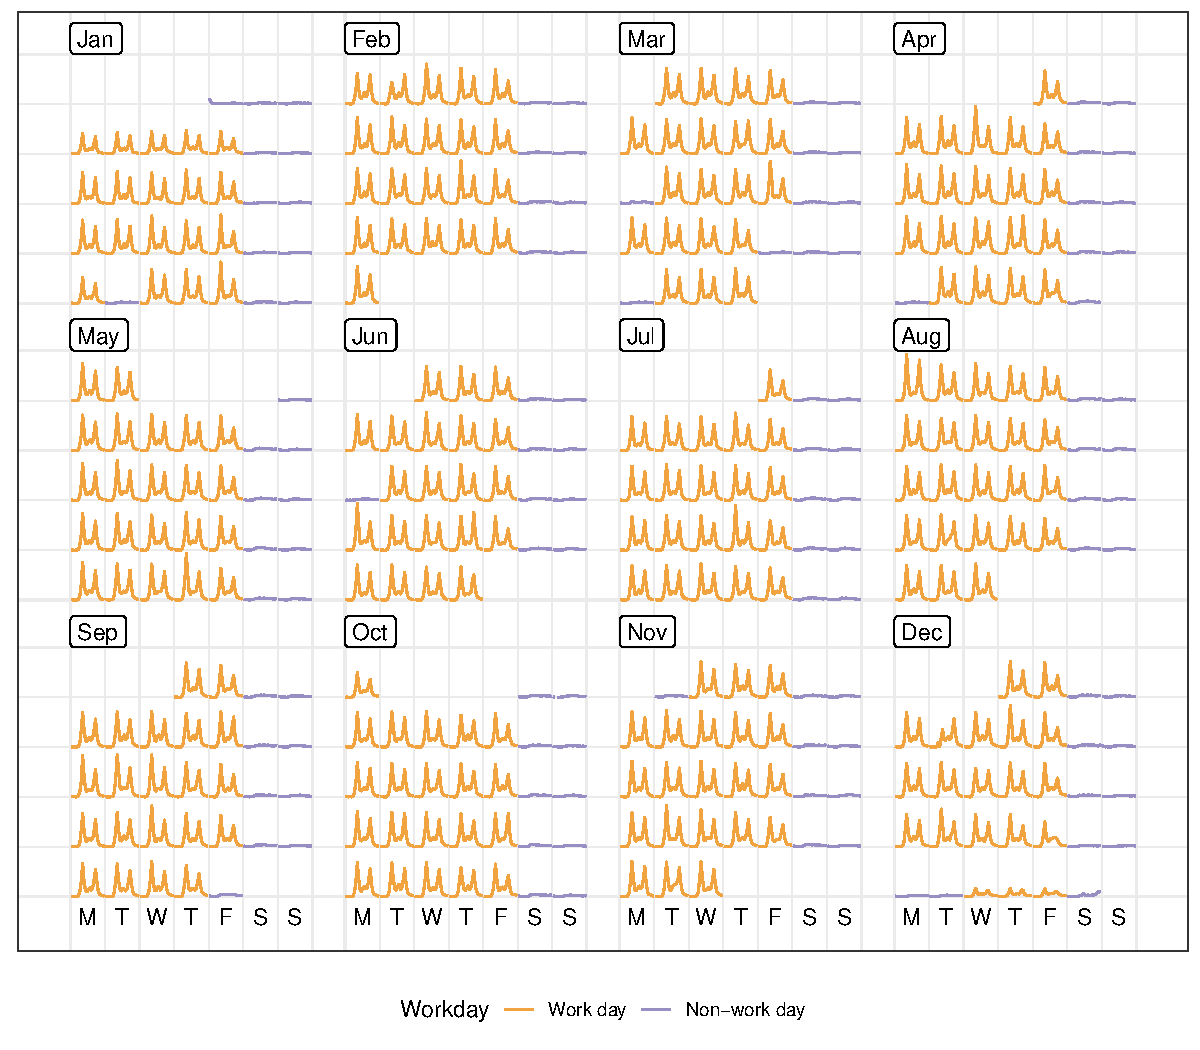
\includegraphics[width=\textwidth]{figure/fs-2016-1} 

}

\caption{The calendar plot of hourly foot traffic at Flagstaff Station ranging from 0 to 6952, using line graphs. The disparities between weekday and weekend along with public holiday, are immediately apparent. The arrangement of the data into a \(3 \times 4\) monthly grid represents all the traffic in 2016. Note that the algorithm wraps the last few days in the sixth week to the top row of each month block for a compact layout, which occurs in May and October.}\label{fig:fs-2016}
\end{figure}



Figure \ref{fig:fs-2016} shows the line graphs framed in the monthly calendar over the year 2016. This is achieved by the \texttt{frame\_calendar()} function, which computes the coordinates on the calendar for the input data variables. These can then be plotted using the usual \textbf{ggplot2} R package \citep{R-ggplot2}. Thus, the grammar of graphics can be applied.

In order to make calendar-based graphics more accessible and informative, reference lines dividing each cell and block, as well as labels indicating weekday and month are also computed before plot construction.

Regarding the monthly calendar, the major reference lines separate every month panel and the minor ones separate every cell, represented by the thick and thin lines in Figure \ref{fig:fs-2016}, respectively. The major reference lines are placed surrounding every month block: for each \(m\), the vertical lines are determined by \(\min{(x)}\) and \(\max{(x)}\); for each \(n\), the horizontal lines are given by \(\min{(y)}\) and \(\max{(y)}\). The minor reference lines are only placed on the left side of every cell: for each \(i\), the vertical division is \(\min{(x)}\); for each \(j\), the horizontal is \(\min{(y)}\).

The month labels located on the top left using \((\min{(x)}, \max{(y)})\) for every \((m, n)\). The weekday texts are uniformly positioned on the bottom of the whole canvas, that is \(\min{(y)}\), with the central position of a cell \(x / 2\) for each \(j\).

\hypertarget{sec:opt}{%
\subsection{Options}\label{sec:opt}}

The algorithm has several optional parameters that modify the layout, direction of display, scales, plot size and switching to polar coordinates. These are accessible to the user by the inputs to the function \texttt{frame\_calendar()}:

\begin{Shaded}
\begin{Highlighting}[]
\KeywordTok{frame_calendar}\NormalTok{(data, x, y, date, }\DataTypeTok{calendar =} \StringTok{"monthly"}\NormalTok{, }\DataTypeTok{dir =} \StringTok{"h"}\NormalTok{,}
  \DataTypeTok{week_start =} \DecValTok{1}\NormalTok{, }\DataTypeTok{nrow =} \OtherTok{NULL}\NormalTok{, }\DataTypeTok{ncol =} \OtherTok{NULL}\NormalTok{, }\DataTypeTok{polar =} \OtherTok{FALSE}\NormalTok{, }\DataTypeTok{scale =} \StringTok{"fixed"}\NormalTok{,}
  \DataTypeTok{width =} \FloatTok{0.95}\NormalTok{, }\DataTypeTok{height =} \FloatTok{0.95}\NormalTok{, }\DataTypeTok{margin =} \OtherTok{NULL}\NormalTok{)}
\end{Highlighting}
\end{Shaded}

It is assumed that the \texttt{data} is in tidy format \citep{wickham2014tidy}, and \texttt{x}, \texttt{y} are the variables that will be mapped to the horizontal and vertical axes in each cell. For example in Figure \ref{fig:fs-2016}, the \texttt{x} is the time of the day, and \texttt{y} is the count. The \texttt{date} argument specifies the date variable in the data, facilitating the range of dates plotted in the calendar layout.

The algorithm handles displaying a single month or several years. The arguments \texttt{nrow} and \texttt{ncol} specify the layout of multiple months. For some time frames, some arrangements may be more beneficial than others. For example, to display data for three years, setting \texttt{nrow\ =\ 3} and \texttt{ncol\ =\ 12} would show each year on a single row.

\hypertarget{layouts}{%
\subsubsection{Layouts}\label{layouts}}

The monthly calendar is the default, but two other formats, weekly and daily, are available with the \texttt{calendar} argument. The daily calendar arranges days along a row, one row per month. The weekly calendar stacks weeks of the year vertically, one row for each week, and one column for each day. The reader can scan down all the Mondays of the year, for example. The daily layout puts more emphasis on day of the month. The weekly calendar is appropriate if most of the variation can be characterized by days of the week. On the other hand, the daily calendar should be used when there is a yearly effect but not a weekly effect in the data (for example, weather data). When both effects are present, the monthly calendar would be a better choice. Temporal patterns motivate which variant should be employed.

\hypertarget{orientation}{%
\subsubsection{Orientation}\label{orientation}}

By default, grids are laid out horizontally. This can be transposed by setting the \texttt{dir} parameter to \texttt{"v"}, in which case \(i\) and \(j\) are swapped in Equation \eqref{eq:grid}. This can be useful for creating calendar layouts for countries where vertical layout is the convention.

\hypertarget{start-of-the-week}{%
\subsubsection{Start of the week}\label{start-of-the-week}}

The start of the week for a monthly calendar is adjustable. The default is Monday (\texttt{1}), which is chosen from the data perspective. The week, however, can begin with Sunday (\texttt{7}) as commonly used in the US and Canada, or other weekday, subject to different countries and cultures.

\hypertarget{polar-transformation}{%
\subsubsection{Polar transformation}\label{polar-transformation}}

When \texttt{polar\ =\ TRUE}, a polar transformation is carried out on the data. The computation is similar to the one described in \citet{Wickham2012glyph}. This produces star glyphs \citep{chambers2017graphical}, where time series lines are transformed in polar coordinates, embedded in the monthly calendar layout. It is most useful in exhibiting cyclical patterns in the data.



\hypertarget{scales}{%
\subsubsection{Scales}\label{scales}}

By default, global scaling is done for values in each plot, with the global minimum and maximum used to fit values into each cell. If the emphasis is on comparing trend rather than magnitude, it is useful to scale locally. For temporal data, this would harness the temporal components. The choices include: free scale within each cell (\texttt{free}), cells derived from the same day of the week (\texttt{free\_wday}), or cells from the same day of the month (\texttt{free\_mday}). The scaling allows for the comparisons of absolute or relative values, and the emphasis of different temporal variations.

With local scaling, the overall variation gives way to the individual shape. Figure \ref{fig:fs-free} shows the same data as Figure \ref{fig:fs-2016}, scaled locally using \texttt{scale\ =\ "free"}. The daily trends are magnified.

\begin{figure}

{\centering 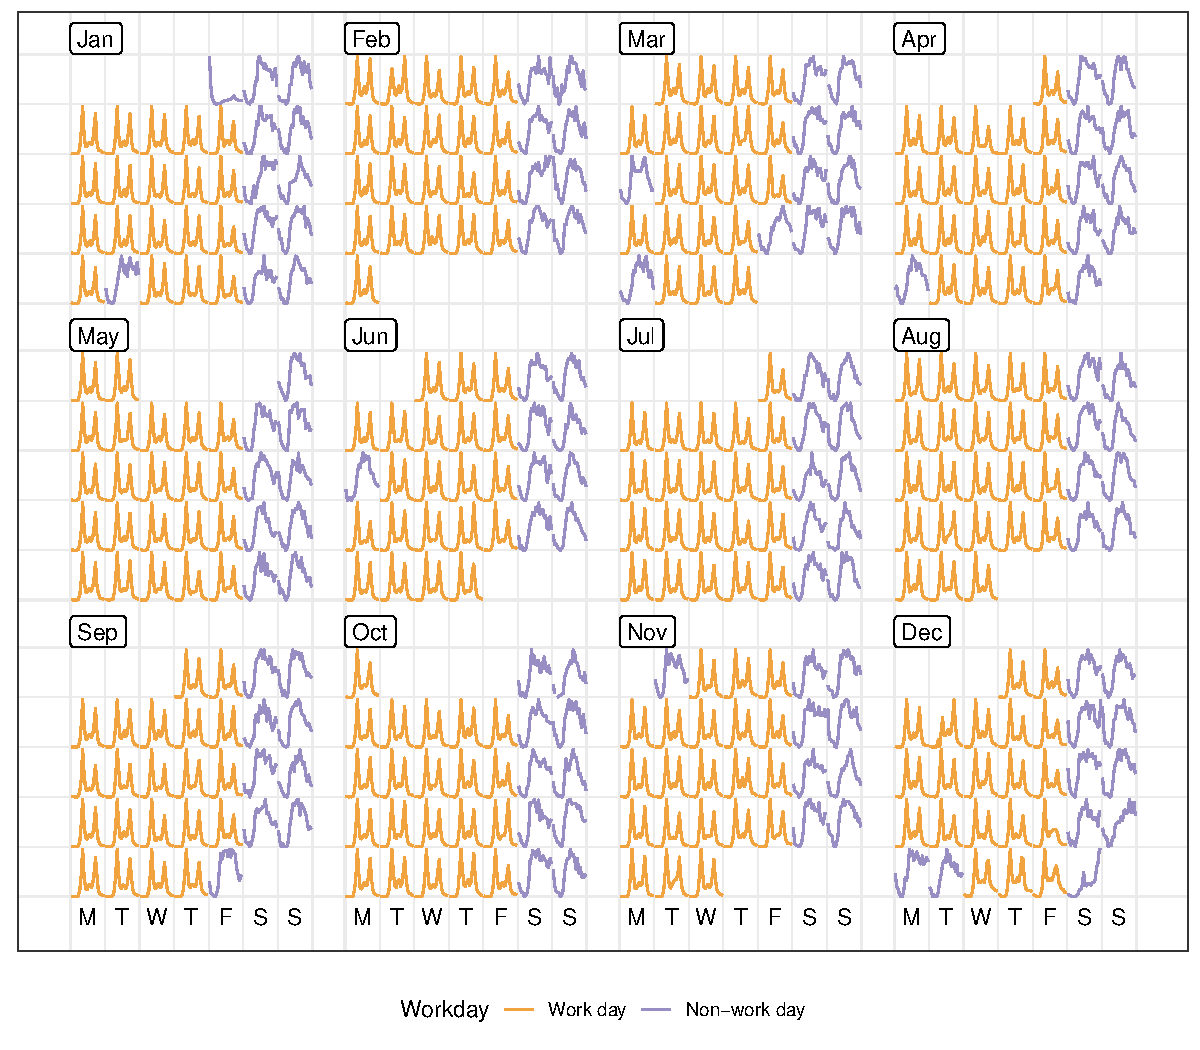
\includegraphics[width=\textwidth]{figure/fs-free-1} 

}

\caption{Line graphs on the calendar format showing hourly foot traffic at Flagstaff Station, scaled individually by day. The shape on a single day becomes more distinctive, as compared to Figure \ref{fig:fs-2016}.}\label{fig:fs-free}
\end{figure}



The \texttt{free\_wday} scales each weekday together. It can be useful to compare trends across weekdays, allowing relative patterns for weekends versus weekdays to be examined. Similarly, the \texttt{free\_mday} uses free scaling for any day within a given month.

\hypertarget{language-support}{%
\subsubsection{Language support}\label{language-support}}

Most countries have adopted this western calendar layout, while the languages used for weekday and month would be different across countries. Other language specifications than English, for text labeling, are available.

\hypertarget{sec:variations}{%
\subsection{Varieties of calendar display}\label{sec:variations}}

\hypertarget{information-overlay}{%
\subsubsection{Information overlay}\label{information-overlay}}

Plots can be layered. A comparison of sensors can be done by overlaying them in the same calendar pane. Figure \ref{fig:overlay} overlays the pedestrian counts for three locations on the same calendar. Differences between the pedestrian patterns at these locations can be more directly compared. For example, the magnitude of the difference in pedestrians at Flagstaff Station at peak hours of commuter can be seen. The big peak in pedestrian counts for special events at Birrarung Marr is clear. Birrarung Marr has a very distinct temporal pattern relative to the other two locations. The nighttime events, such as White Night (third Saturday in February), only affects the foot traffic at the State Library and Birrarung Marr.

\begin{figure}

{\centering 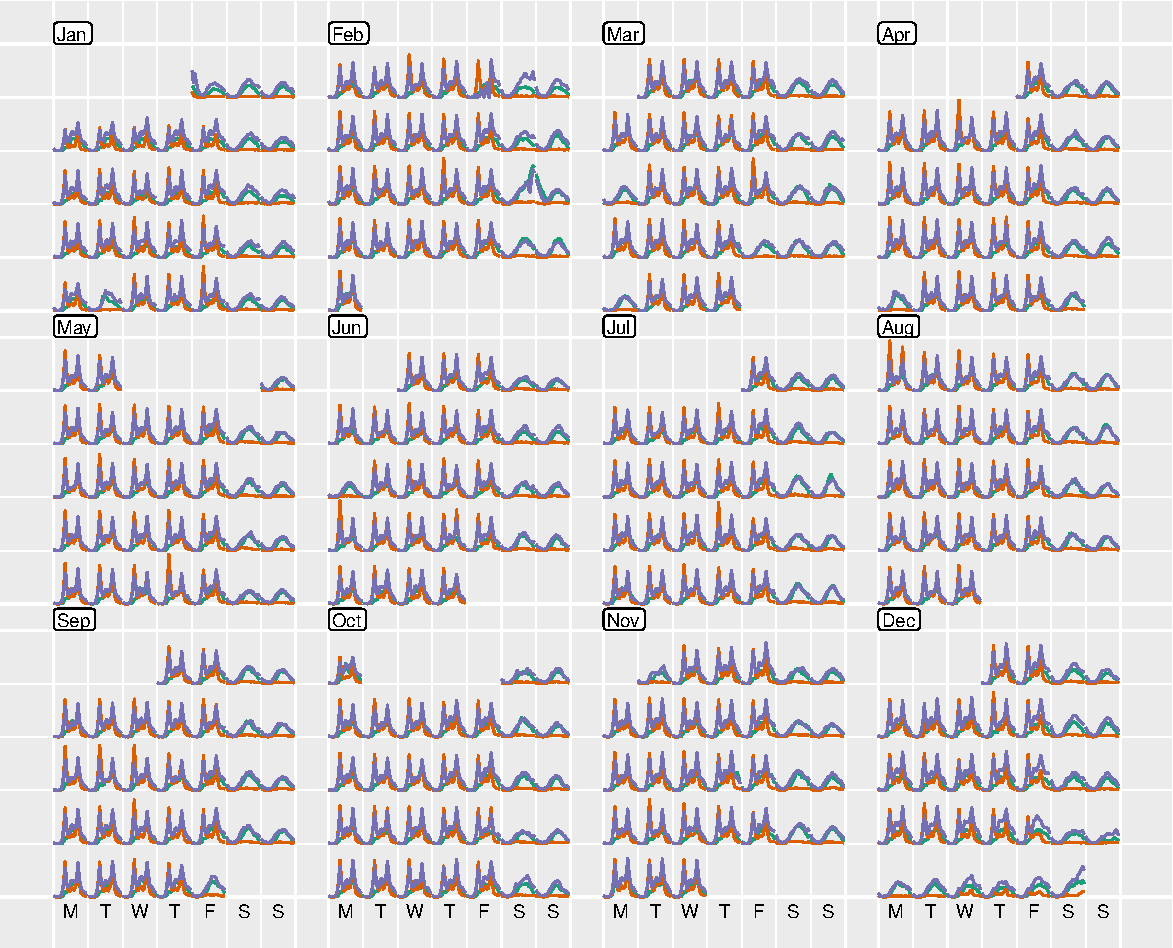
\includegraphics[width=\textwidth]{figure/overlay-1} 

}

\caption{Overlaying line graphs of the three sensors in the monthly calendar, to enable a direct comparison of the counts at three locations. They have very different traffic patterns. Birrarung Marr tends to attract large numbers of pedestrians for special events typically held on weekends, contrasting to the bimodal massive peaks showing commuting traffic at Flagstaff Station.}\label{fig:overlay}
\end{figure}



\hypertarget{faceting-by-covariates}{%
\subsubsection{Faceting by covariates}\label{faceting-by-covariates}}

To avoid overlapping, when differences between groups are large enough to be seen separately, the calendar layout can be faceted into a series of subplots for the different sensors. Figure \ref{fig:facet} shows calendar plots that are faceted by sensors. This arrangement allows comparison of the overall structure between sensors, while emphasizing individual sensor variation. In particular, it can be immediately learned that Birrarung Marr was busy and packed over many weekends, but events took place on Friday evenings only in September. The Australian Open, a major international tennis tournament, attracted constant foot traffic in the last two weeks of January. The calendar plot can be faceted by any categorical variable in the data.

\begin{figure}

{\centering 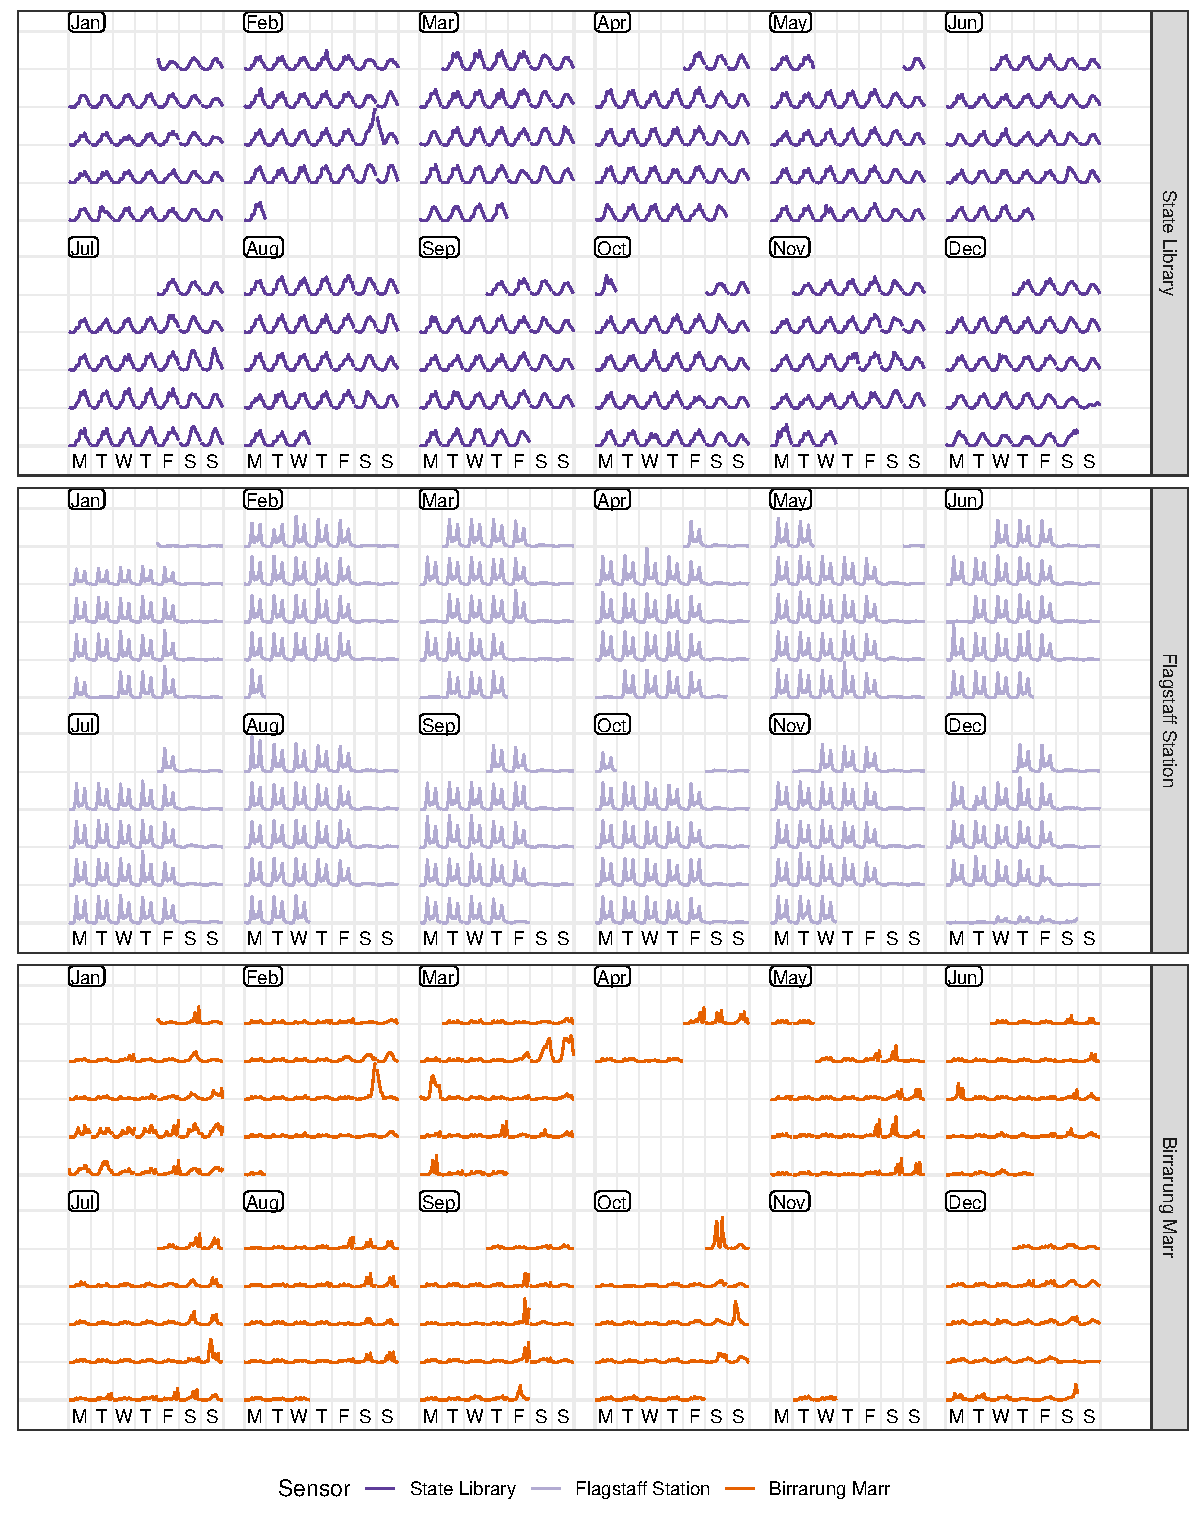
\includegraphics[width=\textwidth]{figure/facet-1} 

}

\caption{Line graphs, embedded in the \(6 \times 2\) monthly calendar, colored and faceted by the 3 sensors. The variations of an individual sensor are emphasized.}\label{fig:facet}
\end{figure}



\hypertarget{different-types-of-plots}{%
\subsubsection{Different types of plots}\label{different-types-of-plots}}

Almost any type of plot can be shown in a calendar pane. Most of the full range of plotting capabilities in \textbf{ggplot2} is available. An example is shown in Figure \ref{fig:scatterplot}: the panes contain lag scatterplots, constructed with local scaling for each day at Flagstaff Station, where the lagged hourly count is assigned to the \texttt{x} argument and the current hourly count to the \texttt{y} argument. It indicates strong autocorrelation on weekends, and weak autocorrelation on work days. The V-shape in the weekday graphs arises when the next hour sees a substantial increase or decrease in counts.

\begin{figure}

{\centering 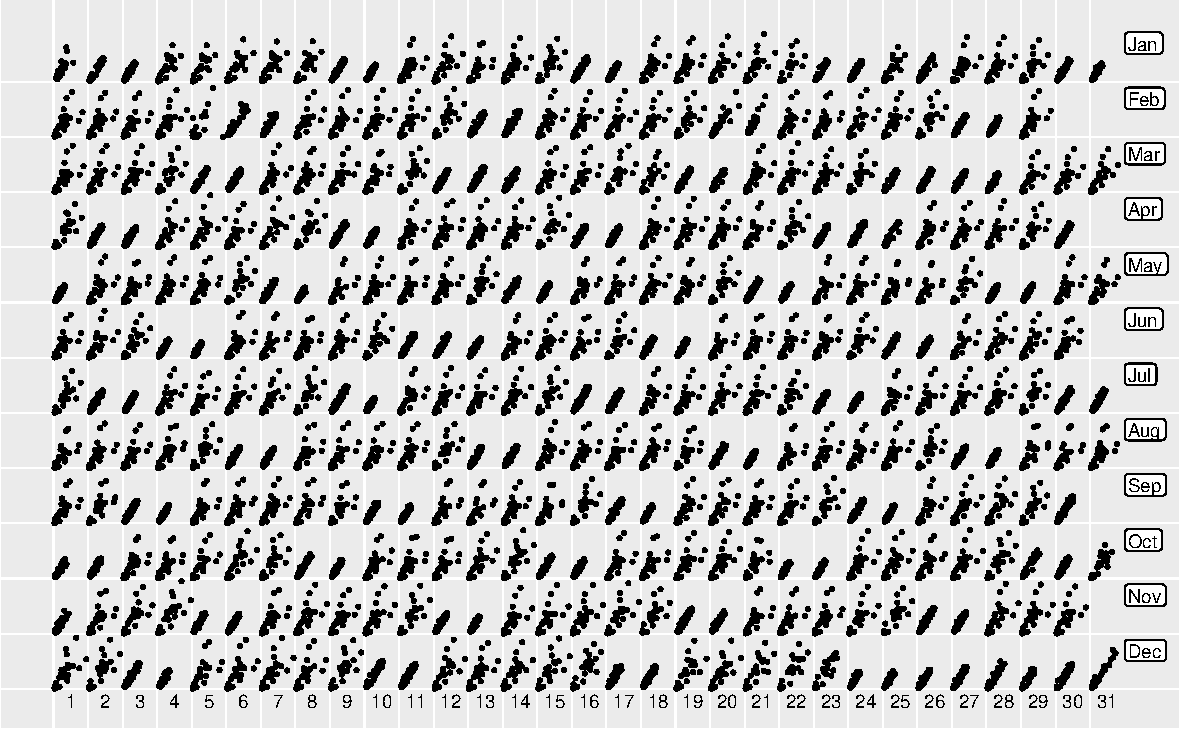
\includegraphics[width=0.75\linewidth]{figure/scatterplot-1} 

}

\caption{Lag scatterplots, with local scaling, in the weekly calendar layout. Each hour's count is plotted against the previous hour's count at Flagstaff Station, to demonstrate the autocorrelation at lag 1. The correlation between them is more consistent on non-work days (blue) than work days (red).}\label{fig:scatterplot}
\end{figure}



The algorithm can also produce more complicated plots, such as boxplots. Figure \ref{fig:chn} uses a loess smooth line \citep{cleveland1979loess} superimposed on side-by-side boxplots. It shows the distribution of hourly counts across all 43 sensors during December. The last week of December is the holiday season: people are off work on the day before Christmas (December 24), go shopping on the Boxing day (December 26), and stay out for the fireworks on New Year's Eve. The text in the plot is labeled in Chinese, showcasing the support for other languages.

\begin{figure}

{\centering 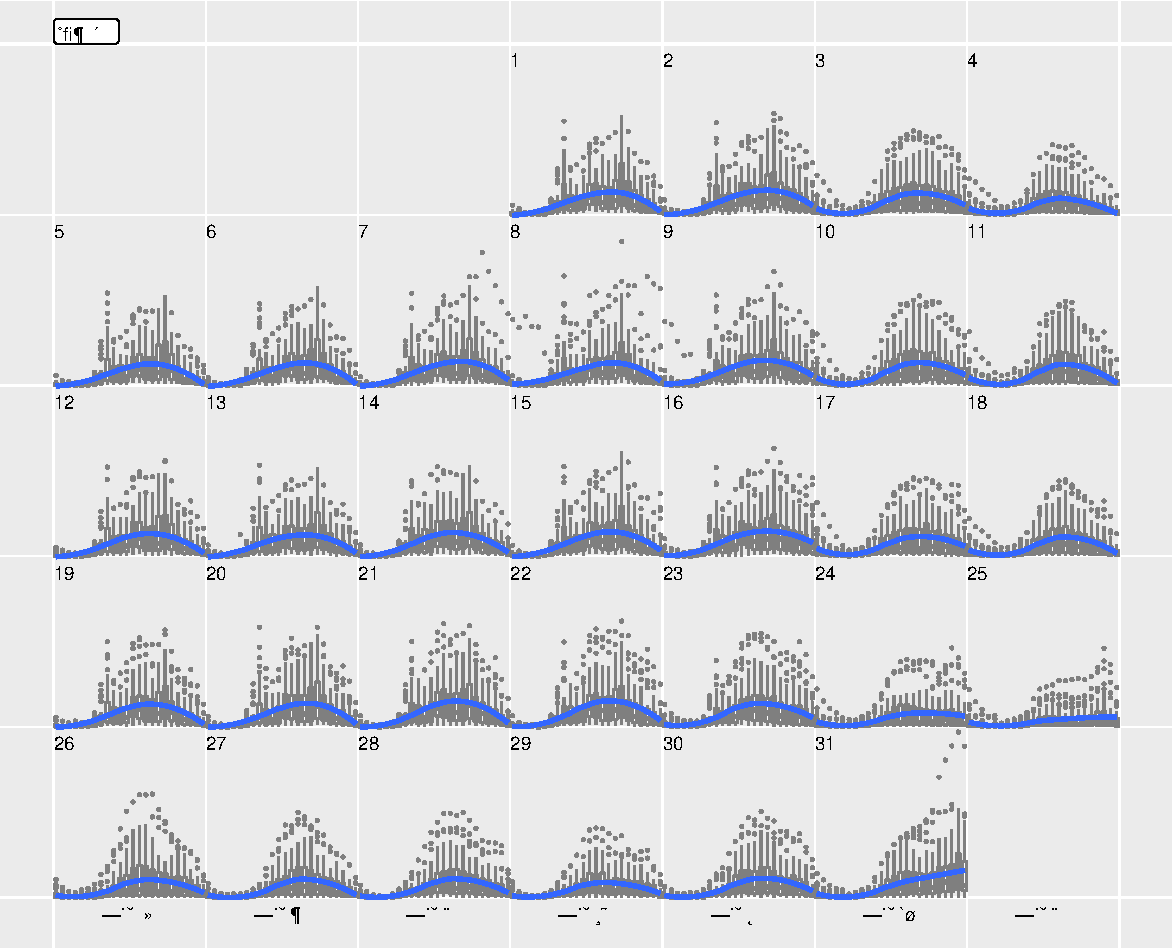
\includegraphics[width=\textwidth]{figure/chn-1} 

}

\caption{Side-by-side boxplots of hourly counts for all the 43 sensors in December 2016, with the loess smooth line superimposed on each day. It shows the hourly distribution in the city as a whole. The increased variability is notable on the last day of December as New Year's Eve approaches. The month and weekday are labeled in Chinese, which demonstrates the support for languages other than English.}\label{fig:chn}
\end{figure}



\hypertarget{interactivity}{%
\subsubsection{Interactivity}\label{interactivity}}

The previous calendar plots are static, made with \textbf{ggplot2}. The interactivity of calendar-based displays can be easily enabled, as long as the interactive graphics system remains true to the spirit of the grammar of graphics, for example, \textbf{plotly} \citep{plotly} in R. As a standalone display, an interactive tooltip can be added to show labels when mousing over a point in the calendar plot, for example the hourly count with the time of day. It is difficult to sense the values from the static display, but the tooltip makes it possible. Options in the \texttt{frame\_calendar()} function can be ported to a form of selection button or text input in a graphical user interface like R shiny \citep{R-shiny}. The display will update on the fly accordingly, via clicking or text input, as desired.

Linking calendar displays to other types of charts is valuable to visually explore the relationships between variables. An example can be found in the \textbf{wanderer4melb} shiny application \citep{R-wanderer4melb}. The calendar most naturally serves as a tool for date selection: by selecting and brushing the glyphs in the calendar, it subsequently highlights the elements of corresponding dates in other time-based plots. The linking between weather data and calendar displays is achieved using the common dates.

\hypertarget{sec:facet-calendar}{%
\subsubsection{Faceted calendar}\label{sec:facet-calendar}}

The \texttt{frame\_calendar()} function described in Section \ref{sec:opt} is a data restructuring function, neatly integrating into a data pipeline but it requires two steps: data transformation and then plot. There is also little freedom to tailor axes and labels, because specialist code needs to be applied.

The \texttt{facet\_calendar()} integrates the algorithm into the \textbf{ggplot2} graphical system so that the calendar layout is automatic, and the full functionality of axes, labels, and customization is accessible. A faceting method lays out panels in a grid. The user needs to supply the variable containing dates, in order for the faceting calendar function to prepare the arrangement of panels, as defined by Equation \eqref{eq:grid}. The remainder of the plot construction for each panel is handled entirely by \textbf{ggplot2} internals.

Formal axes and labels unavailable in calendar plots generated by the \texttt{frame\_calendar()} are possible (Figure \ref{fig:facet-calendar}). It is much easier for readers to infer the scaling (global or local) employed for the plot. Non-existing panels mean non-existing days in the month, and blank panels indicate missing data on the day. This avoids confusion about missing data or days when missingness lives in the ends of month panels, which may occur when using \texttt{frame\_calendar()}.

\begin{figure}

{\centering \includegraphics[width=\textwidth]{figure/facet-calendar-1} 

}

\caption{A faceted calendar showing a fraction of the data shown in Figure \ref{fig:overlay}. The faceted calendar takes more plot real estate than the calendar plot, but it provides native \textbf{ggplot2} support for labels and axes.}\label{fig:facet-calendar}
\end{figure}



However, the \texttt{facet\_calendar()} takes much more run time compared with \texttt{frame\_calendar()}. The faceted calendar also uses more plot real estate for panel headings and axes. The reader can compare the two approaches by examining the compact Figure \ref{fig:overlay}, relative to Figure \ref{fig:facet-calendar}. The space consumed by the former shows a full year, and the latter shows four months, only a third of the data. For fast rendering and economy of space, \texttt{frame\_calendar()} is recommended.

\hypertarget{reasons-to-use-calendar-based-graphics}{%
\subsection{Reasons to use calendar-based graphics}\label{reasons-to-use-calendar-based-graphics}}

The purpose of the calendar display is to facilitate quick discoveries of unusual patterns in people's activities, which is consistent with why analysts should and do use data visualization. It complements the traditional graphical toolbox used to understand general trends, and better profiles vivid and detailed data stories about the way we live. Comparing the conventional displays (Figure \ref{fig:time-series-plot} and \ref{fig:facet-time}) with the new display (Figure \ref{fig:facet}), it can be seen that the calendar display is more informatively compelling: when special events happened, and on what day of the week, and whether they were day or night events. For example, Figure \ref{fig:facet} informs the reader that many events were held in Birrarung Marr on weekend days, while September's events took place on Friday evenings, which is difficult to discern from conventional displays.

\hypertarget{sec:case}{%
\section{Case study}\label{sec:case}}

The use of the calendar display is illustrated on smart meter energy usage from four households in Melbourne, Australia. Individuals can download their own data from the energy supplier, and the data used in this section is sourced from four colleagues of the authors. The calendar display is useful to help people understand their energy use. The data contains half-hourly electricity consumption in the first half of 2018. The analysis begins by looking at the distribution over days of week, then time of day split by work days and non-work days, followed by the calendar display to inspect the daily schedules.

Figure \ref{fig:hod} shows energy consumption against time of day, separately by weekday and weekend. Household 1 is an early riser, starting their day before 6 and going back home around 18 on weekdays. They switch air conditioning on when they get home from work and keep it operating until midnight, evident from the small horizontal cluster of points around 0.8 kWh. On the other hand, the stripes above 1 kWh for household 2 indicates that air conditioning may run continuously for some periods, consuming twice the energy as household 1. A third peak occurs around 15 for household 3 only, likely coinciding when the children arrive home from school. They also have a consistent energy pattern between weekdays and weekends. As for household 4, their home routine starts after 18 on weekdays. Figures \ref{fig:hod}, part of a traditional graphical toolkit, are useful for summarizing overall deviations across days and households.

\begin{figure}

{\centering 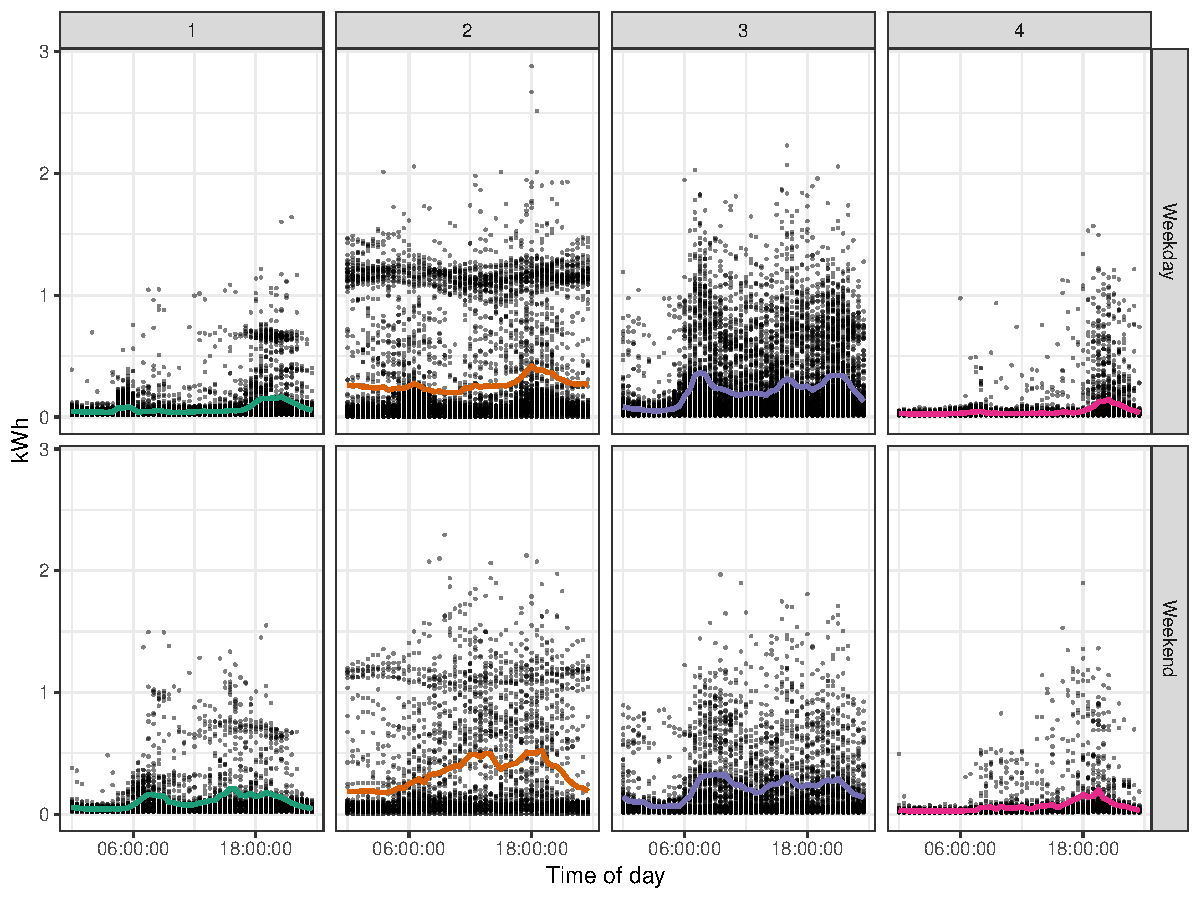
\includegraphics[width=\textwidth]{figure/hod-1} 

}

\caption{Examining sub-daily variability of energy usage by time of day, with hourly averages overlaid, faceted by household and type of day. On weekdays, household 1 wakes up early before 6, and household 2 around 6, followed by household 3 and 4. The use of air conditioning is notable in households 1 and 2, as seen by horizontal clusters of points.}\label{fig:hod}
\end{figure}



\begin{figure}

{\centering \includegraphics[width=\textwidth]{figure/calendar-elec-1} 

}

\caption{Calendar displays faceted by each household using global scales. Long flat low energy usage indicates vacation time, and high energy consumption by household 2 is visible in January and February. Note that April 30 is wrapped to the start of the month.}\label{fig:calendar-elec}
\end{figure}



Figure \ref{fig:calendar-elec} displays the global scaling of each household's data in a calendar layout, unfolding their day-to-day life via electricity usage. Glancing over household 1, their overall energy use is relatively low. Their weekday energy use is distinguishable from their weekends, indicating a working household. The air conditioner appears to be used in the summer months (January and February) for a couple of hours in the evening and weekends. In contrast, household 2 keeps a cooling system functioning for much longer hours, which becomes more evident from late Wednesday through Thursday to early Friday in mid-January. These observations help to explain the stripes and clusters of household 2 in Figure \ref{fig:hod}. It is difficult to give a succinct description of household 3 since everyday energy pattern is variable, but May and June see more structure than the previous months. Individual data can be idiosyncratic, hence aggregated plots like Figure \ref{fig:dow} and \ref{fig:hod} are essential for assembling pieces to form a picture. However, the calendar plots tell the stories that are untold by previous plots, for example, their vacation time. Household 1 is on vacation over three weeks of mid-June, and household 2 also took some days off in the second week of June. Further, household 3 takes one short trip in January and another one starting in the fourth week of June. Household 4 is away over two or three weeks in early April and late June. They all tend to take breaks during June probably due to the fact that the University winter break starts in June.

\hypertarget{sec:discussion}{%
\section{Discussion}\label{sec:discussion}}

The calendar-based visualization provides data plots in the familiar format of an everyday tool. Patterns relating to special events and public holidays for the region are more visible to the viewer.

The calendar layout will be useful for studying consumer trends and human behavior. It will be less useful for physical processes such as weather. The layout does not replace traditional displays, but serves to complement them to further tease out structure in temporal data. Analysts would still be advised to plot overall summaries and deviations in order to study general trends.

The methodology creates the western calendar layout, because most countries have adopted this format. The main difference between countries is the use of different languages for labeling, which is supported by the software. Formats beyond the western calendar, or six-weeks and tetris-like layouts could be achieved by slightly tweaking the modular arithmetic approach. These features will be added as new options in the future.

\hypertarget{acknowledgements}{%
\section*{Acknowledgements}\label{acknowledgements}}
\addcontentsline{toc}{section}{Acknowledgements}

We would like to thank Stuart Lee and Heike Hofmann for their feedback on earlier versions of this work. We thank Thomas Lin Pedersen for pointing out some critical \textbf{ggplot2} internals, which makes the \texttt{facet\_calendar()} implementation possible. We are very grateful to anonymous reviewers for helpful comments that have led to many improvements of the paper. The \textbf{sugrrants} R package is available from CRAN \url{https://CRAN.R-project.org/package=sugrrants} and the development version is available on Github \url{https://github.com/earowang/sugrrants}. All materials required to reproduce this article and a history of the changes can be found at the project's Github repository \url{https://github.com/earowang/paper-calendar-vis}.

\bibliographystyle{agsm}
\bibliography{bibliography.bib}

\end{document}
